\section{A polyhedral piecewise affine model}

In the Godunov scheme (\ref{eq:rhoGodunov}), the update of the density $\rho^{t+1}_{i}$ at cell $i$ depends on the triplet $(\rho^{t}_{i-1}, \rho^{t}_{i}, \rho^{t}_{i+1})$. With $\frac{\Delta t}{\Delta x}=\alpha$, the Godunov scheme reads as:

\begin{equation} \label{eq:rhoGodunov2}
\rho^{t+1}_{i} = \rho^{t}_{i} - \alpha\left(G(\rho^{t}_{i},\rho^{t}_{i+1})-G(\rho^{t}_{i-1},\rho^{t}_{i})\right)
\end{equation}

\subsection{Decomposition in different ``modes''}\label{sec:decompositionModes}

$\rho^{t+1}_{i}$ depends on whether both pairs $(\rho^{t}_{i-1}, \rho^{t}_{i})$ and $(\rho^{t}_{i}, \rho^{t}_{i+1})$ are in \textbf{W}, \textbf{L}, or \textbf{D} via $G(\rho^{t}_{i-1},\rho^{t}_{i})$ and $G(\rho^{t}_{i},\rho^{t}_{i+1})$. So there are nine possible combinations at cell $i$, which can be reduced to seven ''modes'' since the pairs $(\rho^{t}_{i-1}, \rho^{t}_{i})$ and $(\rho^{t}_{i}, \rho^{t}_{i+1})$ have $\rho^{t}_{i}$ in common. Let's denote by $f(\rho^{t}_{i-1},\rho^{t}_{i},\rho^{t}_{i+1})$ and $f_{DN}(\rho^{t}_{i-1},\rho^{t}_{i},\rho^{t}_{i+1})$ the vector functions for $\rho^{t+1}_{i}$ for the general and the Danganzo-Newell cases respectively, which variables are $\rho^{t}_{i-1}$, $\rho^{t}_{i}$, and $\rho^{t}_{i+1}$. Table \ref{table:modes} list these seven possibilities, which can be easily derived from Figure \ref{fig:godunovDiagram}.

\begin{table}[here]
\centering % used for centering table
\begin{tabular}{c c c c} % centered columns (4 columns)
\hline\hline %inserts double horizontal lines
Mode & $(\rho^{t}_{i-1}, \rho^{t}_{i})$ & $(\rho^{t}_{i}, \rho^{t}_{i+1})$ & $f(\rho^{t}_{i-1},\rho^{t}_{i},\rho^{t}_{i+1})$ \\ [0.5ex]% inserts table
%heading
\hline % inserts single horizontal line
1 & W & W & $\rho^{t}_{i} - \alpha(R(\rho^{t}_{i+1})-R(\rho^{t}_{i}))$ \\ [1ex]
2 & W & L & $\rho^{t}_{i} - \alpha(q_{c}-R(\rho^{t}_{i}))$ \\ [1ex]
3 & L & W & $\rho^{t}_{i} - \alpha(R(\rho^{t}_{i+1})-q_{c})$ \\ [1ex]
4 & L & D & $\rho^{t}_{i} - \alpha(S(\rho^{t}_{i})-q_{c})$ \\ [1ex]
5 & D & W & $\rho^{t}_{i} - \alpha(R(\rho^{t}_{i+1})-S(\rho^{t}_{i-1}))$ \\ [1ex]
6 & D & L & $\rho^{t}_{i} - \alpha(q_{c}-S(\rho^{t}_{i-1}))$ \\ [1ex]
7 & D & D & $\rho^{t}_{i} - \alpha(S(\rho^{t}_{i})-S(\rho^{t}_{i-1}))$ \\ [1ex]% [1ex] adds vertical space
\hline %inserts single line
\end{tabular}
\caption{Different modes of $\rho^{t+1}_{i} = f(\rho^{t}_{i-1},\rho^{t}_{i},\rho^{t}_{i+1})$ depending on the values of $G(\rho^{t}_{i-1},\rho^{t}_{i})$ and $G(\rho^{t}_{i},\rho^{t}_{i+1})$ in the space $(\rho_{1},\rho_{2})$.}
\label{table:modes} % is used to refer this table in the text
\end{table}

\begin{table}[here]
\centering % used for centering table
\begin{tabular}{c c} % centered columns (4 columns)
\hline\hline %inserts double horizontal lines
Mode & $f_{DN}(\rho^{t}_{i-1},\rho^{t}_{i},\rho^{t}_{i+1})$ \\ [0.5ex]% inserts table
%heading
\hline % inserts single horizontal line
1 & $(1 - \alpha \omega_{f})\rho^{t}_{i} + \alpha \omega_{f} \rho^{t}_{i+1}$ \\ [1ex]
2 & $(1 - \alpha \omega_{f})\rho^{t}_{i} + \alpha \omega_{f} \rho_{c}$ \\ [1ex]
3 & $\rho^{t}_{i} + \alpha \omega_{f}\rho^{t}_{i+1} - \alpha \omega_{f}\rho_{c}$ \\ [1ex]
4 & $(1 - \alpha v_{f})\rho^{t}_{i} + \alpha v_{f} \rho_{c}$ \\ [1ex]
5 & $\alpha v_{f} \rho^{t}_{i-1} + \rho^{t}_{i} + \alpha \omega_{f} \rho^{t}_{i+1} - \alpha \omega_{f} \rho_{\text{jam}}$ \\ [1ex]
6 & $\alpha v_{f} \rho^{t}_{i-1} + \rho^{t}_{i} - \alpha v_{f} \rho_{c}$ \\ [1ex]
7 & $\alpha v_{f} \rho^{t}_{i-1} + (1 - \alpha v_{f})\rho^{t}_{i}$ \\ [1ex]% [1ex] adds vertical space
\hline %inserts single line
\end{tabular}
\label{table:modesDN} % is used to refer this table in the text
\caption{Different values of $\rho^{t+1}_{i} = f_{DN}(\rho^{t}_{i-1},\rho^{t}_{i},\rho^{t}_{i+1})$ for a Daganzo-Newell fundamental diagram.}
\end{table}

For instance, for the first mode, $(\rho^{t}_{i-1}, \rho^{t}_{i})$ and $(\rho^{t}_{i}, \rho^{t}_{i+1})$ are both in \textbf{W} (see Figure \ref{fig:godunovDiagram}), thus $G(\rho^{t}_{i-1}, \rho^{t}_{i}) = R(\rho^{t}_{i})$ and $G(\rho^{t}_{i}, \rho^{t}_{i+1}) = R(\rho^{t}_{i+1})$, and then $\rho^{t+1} = f_{1}(\rho^{t}_{i-1},\rho^{t}_{i},\rho^{t}_{i+1}) = \rho^{t}_{i} - \alpha(R_{+}(\rho^{t}_{i+1})-R(\rho^{t}_{i}))$, where $f_{1}$ is the first entry of $f$. By extending this result to an entire link with discrete state space indexed by $i = 1,\cdots,n$, where $n$ is the number of space steps, we have an exhaustive description of the space of ``modes'' along the link. 

\hspace{10mm}

\noindent \textbf{Remark:} A priori, the number of modes in Table \ref{table:modes} renders the approach of mode decomposition for estimation untractable: for $n$ cells, the number of possible modes at any given time is technically $7^{n}$. Since there is a correlation between two consecutive indices $i$ and $i+1$, the number of modes for the entire link reduces from $7^{n}$ to an expression in the form of $a\cdot\beta^{n} + b\cdot\gamma^{n} + c\cdot\delta^{n}$ which lower and upper bounds are proved to be $3\cdot 2^{n}$ and $3\cdot (2.5)^{n}$ respectively (for full details, see Appendix \ref{sec:modes}). And we will see later in section \ref{sec:implementation} that the implementation of the Kalman filter in each mode has $O(n^{2})$ time complexity and $O(n)$ space complexity.

\hspace{10mm}

We define $J$, the Jacobian matrix of $f$ with respect to $(\rho^{t}_{i-1},\rho^{t}_{i},\rho^{t}_{i+1})$ in each of the modes (which are all linear):

\begin{equation}\label{eq:jacobian}
J = \left(\frac{\partial f_{j}}{\partial \rho_{k}}\right)_{j=1,\cdots,7,k=i-1,i,i+1}
\end{equation}

\noindent Where $f_{j}$ is the $j$-th entry of the vector function $f$ defined in Table \ref{table:modes}. It is useful to make explicit the Jacobian matrix $J_{DN}$ of the vector function $f_{DN}$ with respect to $(\rho^{t}_{i-1},\rho^{t}_{i},\rho^{t}_{i+1})$, and the constant term $w$:

\begin{equation} \label{eq:jacobianDN}
J_{DN} = \left( \begin{array}{ccc}
0 & 1 - \alpha \omega_{f} & \alpha \omega_{f} \\
0 & 1 - \alpha \omega_{f} & 0 \\
0 & 1 & \alpha \omega_{f} \\
0 &  1 - \alpha v_{f} & 0 \\
\alpha v_{f} & 1 & \alpha \omega_{f} \\
\alpha v_{f} & 1 & 0 \\
\alpha v_{f} & 1 - \alpha v_{f} & 0
\end{array} \right)
\end{equation}

\begin{equation}\label{eq:jacobianDN2}
w = \left( \begin{array}{c}
0 \\
\alpha \omega_{f} \rho_{c}\\
-\alpha \omega_{f} \rho_{c}\\
\alpha v_{f} \rho_{c}\\
-\alpha \omega_{f} \rho_{\text{jam}}\\
-\alpha v_{f} \rho_{c}\\
0
\end{array} \right)
\end{equation}

Since $f_{DN}$ is a \textit{linear function} of $(\rho^{t}_{i-1},\rho^{t}_{i},\rho^{t}_{i+1})$ as shown in Table \ref{table:modes}, we can notice that $J_{DN}$ is constant. More notably, the vector function $f_{DN}$ can be rewritten as:

\begin{equation}
\rho^{t+1}_{i} = f_{DN}(\rho^{t}_{i-1},\rho^{t}_{i},\rho^{t}_{i+1}) = J_{DN}\left( \begin{array}{c}
\rho^{t}_{i-1}\\
\rho^{t}_{i}\\
\rho^{t}_{i+1}
\end{array} \right)
+ w
\label{eq:fDN}
\end{equation}

In the next section, we will see that the decomposition in ``modes'' as shown in Table \ref{table:modes} leads to a piecewise affine formulation of the Godunov scheme in the case of the Daganzo-Newell fundamental diagram.


\subsection{Polyhedral piecewise affine formulation}\label{sec:formulation}

Let us consider a link with discrete time step indexed by $t\geq 0$ and discrete space step indexed by $i = 1,\cdots,n$, and let's denote $\boldsymbol\rho^{t} = (\rho^{t}_{0},\rho^{t}_{1},\cdots,\rho^{t}_{n},\rho^{t}_{n+1})$ a $n+2$ dimensional vector which describes the state of the link at time $t$ in the space $\mathcal{S} = [0,\rho_{\text{jam}}]^{n+2}$. $\rho^{t}_{i}$ is the density at time $t$ and cell $i$. We can note that the ghost cells $0$ and $n+1$ are included in the state of the link\footnotemark.

\footnotetext{
The values of $\rho^{t}_{0}$ and $\rho^{t}_{n+1}$ are given by the prescibed boundary conditions to be imposed on the in left and right side of the domain respectively. Note that these boundary values do not always affect the physical domain because of the nonlinear operator \ref{eq:rhoGodunovFlux3}, which causes the boundary conditions to be implemented in the weak sense. For more details, see \cite{Strub2006}.
}

\begin{figure}[ht]
  \centering
    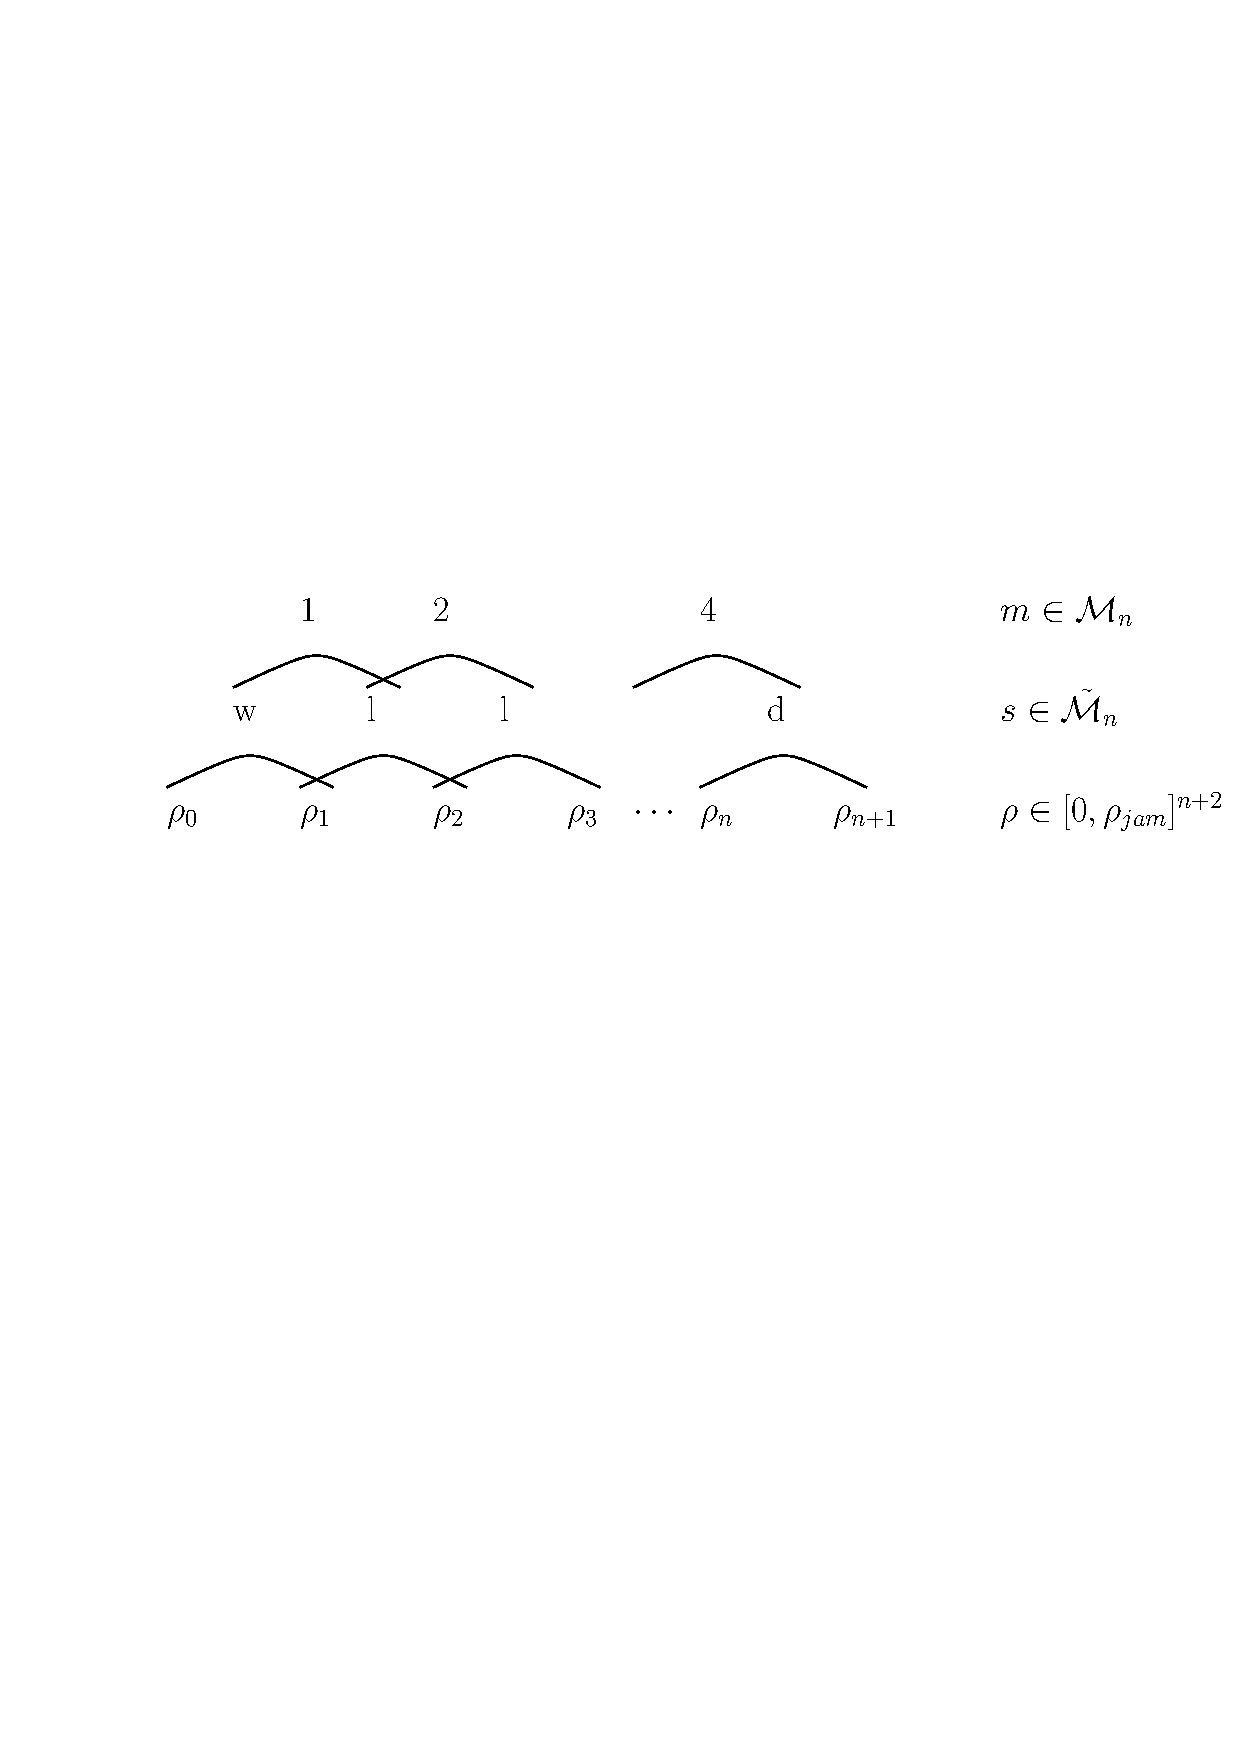
\includegraphics[width=8cm]{figures/modes.pdf}
    \caption{An illustration of the vectors $\boldsymbol \rho\in[0,\rho_{\text{jam}}]^{n+2}$, $\boldsymbol s\in\tilde{\mathcal{M}}_{n}\subset\{\text{w,l,d}\}^{n+1}$, and $\boldsymbol m\in\mathcal{M}_{n}\subset\{1,\cdots,7\}^{n}$ for $n$ cells.}
    \label{fig:modes}
\end{figure}

\noindent\textbf{Definition of the space of modes:} Let us denote by $\mathcal{M}_{n}$ the space of modes ($\mathcal{M}_{n}\subset\{1,\cdots,7\}^{n}$). For $\boldsymbol m \in \mathcal{M}_{n}$, $\boldsymbol m$ is a vector of dimension $n$ for which the $i$-th entry $m_{i}\in\{1,\cdots,7\}$ is the mode at cell $i$. Equivalently, each element of $\mathcal{M}_{n}$ can be described as a sequence of regions in which the pair $(\rho_{i},\rho_{i+1})$ is, for $i=0,\cdots,n$. Hence, we define the equivalent space of modes $\tilde{\mathcal{M}}_{n}\subset\{\text{w,l,d}\}^{n+1}$, and for $\boldsymbol s \in \tilde{\mathcal{M}}_{n}$, $\boldsymbol s$ is a vector of dimension $n+1$ for which the $i$-th entry $s_{i}\in\{\text{w,l,d}\}$ is the region of the pair $(\rho_{i},\rho_{i+1})$, for $i=0,\cdots,n$. As we will see later, this second definition gives a description of the \emph{partition of the space} $\mathcal{S}$ \emph{into different polyhedra} $\textbf{P}_{\boldsymbol m}$ \emph{in which the mode is} $\boldsymbol m$. See Figure \ref{fig:modes} for an illustration.

\hspace{10mm}

The $n$-dimensional vector $\boldsymbol m\in\mathcal{M}_{n}$ describes the mode of the link at amy time, as defined in the previous section. At each time increment, the state of the link is updated through the following nonlinear dynamical system:

\begin{equation}
\boldsymbol\rho^{t+1} = F[\boldsymbol\rho^{t}]
\label{eq:underlyingSystem1}
\end{equation}

\noindent with $F[\cdot]$ a n+2 dimensional function vector. When $\boldsymbol\rho^{t}\in \boldsymbol P_{\boldsymbol m}$ (i.e. the mode at time $t$ is $\boldsymbol m$), and the boundary conditions upstream and downstream at time step $t+1$ are $u^{t+1}$ and $d^{t+1}$, the $i$-th entry $\rho^{t+1}_{i}=F_{i}[\boldsymbol\rho^{t}]$ is:

\begin{equation}
\rho^{t+1}_{i} = \begin{cases}
f_{m_{i}}(\rho^{t}_{i-1},\rho^{t}_{i},\rho^{t}_{i+1}) & \text{for}\quad i=1,...,n\\
u^{t+1} & \text{for}\quad i=0\\
d^{t+1} & \text{for}\quad i=n+1
\end{cases}
\label{eq:underlyingSystem2}
\end{equation}

\noindent where $m_{i}$ denotes the $i$-th entry of $\boldsymbol m \in\mathcal{M}_{n}$, i.e. the mode of cell $i$ at time step $t$. $f_{m_{i}}(\rho^{t}_{i-1},\rho^{t}_{i},\rho^{t}_{i+1})$ is the $m_{i}$-th entry of the function vector $f$ evaluated in $(\rho^{t}_{i-1},\rho^{t}_{i},\rho^{t}_{i+1})$. We note that $\rho^{t+1}_{0}=u^{t+1}$ and $\rho^{t+1}_{n+1}=d^{t+1}$, which means that the ghost cells are the boundary conditions of the CTM. For a Daganzo-Newell fundamental diagram, with $L_{m_{i}}$ the $m_{i}$-th line of $J_{DN}$ and $w_{m_{i}}$ the $m_{i}$-th entry of $w$, the update operator of the dynamical system is:

\begin{equation}
\begin{array}{l}
\rho^{t+1}_{i}\\
= \begin{cases}
L_{m_{i}}.\left( \begin{array}{c}
\rho^{t}_{i-1}\\
\rho^{t}_{i}\\
\rho^{t}_{i+1}
\end{array} \right)
+ w_{m_{i}} & \text{for }i=1,\cdots,n\\
u^{t+1} & \text{for }i=0\\
d^{t+1} & \text{for }i=n+1
\end{cases}
\end{array}
\label{eq:underlyingSystemDN}
\end{equation}

\noindent When $\boldsymbol\rho^{t}\in\textbf{P}_{\boldsymbol m}$, the $(n+2)\times(n+2)$-dimensional state-transition matrix $A_{\boldsymbol m}$ is tridiagonal with diagonal elements $\{0, J_{m_{1},2},...,J_{m_{n},2},0\}$, lower diagonal elements $\{J_{m_{1},1},J_{m_{2},1},...,J_{m_{n},1},0\}$, and upper diagonal elements $\{0,J_{m_{1},3},J_{m_{2},3},...,J_{m_{n},3}\}$ where $J$ (or $J_{DN}$) are defined in equations (\ref{eq:jacobian}), (\ref{eq:jacobianDN}). Equivalently:

\begin{equation}\label{eq:matrixA}
 A_{\boldsymbol m} =
 \begin{pmatrix}
0 & \cdots & 0 \\
L_{m_{1}} & & \\
& \ddots & \\
& & L_{m_{n}}\\
0 & \cdots & 0
\end{pmatrix}
\end{equation}

\noindent Let us denote $b_{\boldsymbol m}$ and $c_{t+1}$ the two vectors of dimension $(n+2)$ with entries $\{0,w_{m^{t}_{1}},\cdots,w_{m^{t}_{n}},0\}$ and $\{u^{t+1},0,\cdots,$ $0,d^{t+1}\}$ repectively, and $\textbf{P}_{\boldsymbol m}$ the subset of space $\mathcal{S}$ where the mode is $\boldsymbol m$. The update operator of the dynamical system is \emph{piecewise affine}:

\begin{equation}
\boldsymbol\rho^{t+1} = A_{\boldsymbol m} \boldsymbol\rho^{t} + b_{\boldsymbol m} + c_{t+1} \quad\text{if}\quad\boldsymbol\rho^{t}\in\textbf{P}_{\boldsymbol m}
\label{eq:underlyingSystemDN2}
\end{equation}

\noindent We provide now a description of the partition of the space into the polyhedra $\textbf{P}_{\boldsymbol m}$ in which the mode is $\boldsymbol m$. See appendix \ref{sec:polytope} for details on polyhedra and their representation.

\hspace{10mm}

\noindent\textbf{Polyhedral partition of the space:} For a discretization into $n$ cells, we chose to describe the ensemble of modes $\tilde{\mathcal{M}}_{n}$ in sequences $\boldsymbol s \in \{w,l,d\}^{n+1}$ and define $\textbf{P}_{\boldsymbol s}$ the corresponding polyhedron for each sequence. Let us define $3^{n+1}$ polyhedra $\textbf{W}_{i}, \textbf{L}_{i}, \textbf{D}_{i}$ for $i=0,\cdots,n$ in the space $\mathcal{S}$:

\begin{equation}
\begin{array}{ll}
\textbf{W}_{i} & = \{(\rho_{i},\rho_{i+1}) \mid \rho_{i+1} + \frac{v_{f}}{\omega_{f}}\rho_{i} > \rho_{\text{jam}} \text{ ,   } \rho_{i+1} > \rho_{c}\}\\
\textbf{L}_{i} & = \{(\rho_{i},\rho_{i+1}) \mid \rho_{i} > \rho_{c} \text{ ,   } \rho_{i+1} \leq \rho_{c}\}\\
\textbf{D}_{i} & = \{(\rho_{i},\rho_{i+1}) \mid \rho_{i+1} + \frac{v_{f}}{\omega_{f}}\rho_{i} \leq \rho_{\text{jam}} \text{ ,   } \rho_{i} \leq \rho_{c}\}
\end{array}
\label{eq:regions3}
\end{equation}

\noindent Each mode or possible sequence of regions $\boldsymbol s \in \mathcal{M}_{n}$ is valid in a polyhedron $\textbf{P}_{\boldsymbol s}$ that is the intersection of $n+1$ polyhedra:

\begin{equation}
\textbf{P}_{\boldsymbol m}=\bigcap_{i=0}^{n} \textbf{Q}_{i}
\label{eq:Hrepresentation}
\end{equation}

\noindent where the polyhedra $\textbf{Q}_{i}$ are

\begin{equation}
\textbf{Q}_{i}=
\begin{cases}
\textbf{W}_{i} & \text{ if } s_{i}=w\\
\textbf{L}_{i} & \text{ if } s_{i}=l\\
\textbf{D}_{i} & \text{ if } s_{i}=d
\end{cases}
\label{eq:Hrepresentation2}
\end{equation}


Moreover, for two different modes $\boldsymbol s$ and $\boldsymbol s'$, and corresponding polyhedra $\textbf{P}_{\boldsymbol s}=\bigcap_{i=0}^{n} \textbf{Q}_{i}$ and $\textbf{P}_{\boldsymbol s'}=\bigcap_{i=0}^{n} \textbf{Q}'_{i}$, we can find an index $i$ for which $\textbf{Q}_{i}$ and $\textbf{Q}'_{i}$ are disjoint. For instance, suppose without loss of generality that $\textbf{Q}_{i}=\textbf{W}_{i}$ and $\textbf{Q}'_{i}=\textbf{D}_{i}$, and we know that $\textbf{W}_{i}$ and $\textbf{D}_{i}$ are disjoint. Then in this case, the hyperplan $\{\boldsymbol \rho\mid\rho_{i+1} + \frac{v_{f}}{\omega_{f}}\rho_{i} = \rho_{\text{jam}}\}$ is a seperating hyperplan between $\textbf{P}_{\boldsymbol s}$ and $\textbf{P}_{\boldsymbol s'}$. Hence, $\textbf{P}_{\boldsymbol s}$ and $\textbf{P}_{\boldsymbol s'}$ are disjoint and the family $\{\textbf{P}_{\boldsymbol s}\}_{\boldsymbol s \in \mathcal{M}_{n}}$ is a partition of $\mathcal{M}_{n}$.